\title{
	DS-GS 1011 Assignment 2\\
	RNN/CNN-based Nature Language Inference
}
\author{
        Wenting Qi     \quad NetID: wq244\\
}

\documentclass[10pt]{article}
\usepackage[a4paper, total={7in, 11in}]{geometry}
\usepackage{graphicx}
\graphicspath{ {./Assignment2_Image/} }
\usepackage[font=scriptsize]{caption}
\usepackage{mwe}
\usepackage{wrapfig}
\usepackage[export]{adjustbox}
\usepackage{hyperref}

\begin{document}
\maketitle

\begin{abstract}
This paper explores the Standard Nature Language Inference (SNLI) Task through the RNN and CNN approaches model. The dataset contains two sentences, \textit{premise} and \textit{hypothesis}. The goal for the model is to catergorize the relationship of two sentences into three classes \textit{contradicts}, \textit{neutral}, \textit{entails}. The model will be trained using 100,000 instances training set and 1,000 instances validation set providing from Standford SNLI project.
The model takes sentences consisting of pre-embed  word tokens using FastText vector sets as input, applying CNN or RNN model seperately as encoder and interating the two vectors to go through two layer of neural networks and output the required classification.The paper tunes hyperparameters of the RNN and CNN model, including the size of the hidden layers, the method of hidden representations interaction, kernal size(CNN).
In the end, best perform model will be tested on Multi Natural Language Inference(MNLI) task to analyse the influence of genre on language processing.
\end{abstract}

\section{RNN Model}
In this section, the paper will introduce briefly on the data preperatin before the build of RNN model. The paper chooses the bidirectional Gated Recurrent Unit model, which incorperates the whole sentece's environment information for each embedded words. The hyperparameters of hidden size and vecter interaction methods will be varied to experiment on the influence on the model performance. 


\paragraph{Size of Hidden Layers}
To begin, the pre-seperated train data set and validation data set are loaded. Note that the loaded label is in the form of string 'contradict', 'neutral', 'entail'. The paper converted the labels to numercal classes 0, 1, 2 repectively. The word tokens are transfered to indices and sorted in descending length order according to sentence 1 into the dataloader. For dynamic padding in RNN model, the inputs are required to be in descending order. Here, sentence 2 will be sorted within the batch to ensure the matching sentences are in the same batch after automatic shaffle into batches of size of 128.\par

Both sentences will be embedded by looking through the loaded FastText vectors sets. The baseline model \textbf{Model I} takes in the two embedded sentences and concatenates them after encoding them seperately through a one-layer bidirectional GRU model with hidden size of 100. The concatenated vector is then fed into two layers of fully connected neural networks and gives an output of three classes.  We train the model for 5 epochs and the test the accuracy on the validdation set. The model gives its highest accuracy of 62.2\% at the end of the third epoch. \par

\begin{table}[h]
\centering
\caption{Parameters Size for Model I, II, III}
\label{my-label}
\begin{tabular}{llll}
\hline
                     & Model I & Model II & Model III \\ \hline
Number of Parameters & 402803  & 2528403  & 6414003   \\ \hline
\end{tabular}
\end{table}
\begin{figure}[]
\centering
\begin{minipage}{.4\textwidth}
  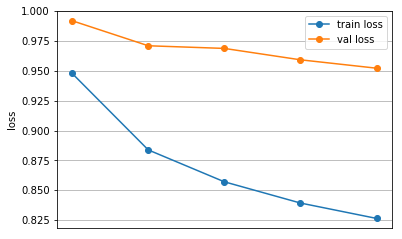
\includegraphics[width=\textwidth]{plot5}
  \caption{Training and Validation Loss for Model I}
\end{minipage}%
\hfill
\begin{minipage}{.4\textwidth}
  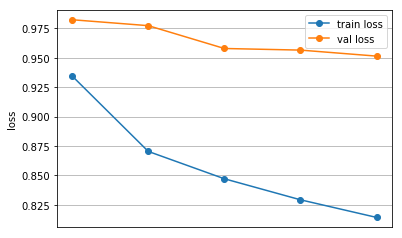
\includegraphics[width=\textwidth]{plot6}
  \caption{Training and Validation Loss for Model II}
\end{minipage}
\end{figure}

The performance of the model is far from satisfying. The paper experiments on various size of hidden layers: size of 300 \textbf{Model II} , the size of 500 \textbf{Model III} . The learning curve for the three models are plotted. Figure 1 shows that as the hidden dimension increases, the performance of the model increases faster and reaches higher accuracy. Thought the final accuracy on the validation set are close, 61.6\%  [Model I], 62.9\%  [Model II], 62.2\%  [Model III], \textbf{Model III}  with the has the higher accuracy through most of the time and yields the highest accuracy among all at 63.6\% at epoch 5. Figure 1-3 shows the validation loss and train loss curve for the Model I, II, II respectively.
 Figure 5 also shows that as the hidden size increases, the performance of the model tends to be more volatile. It is suspected that the increase in the number of parameters causes the irregularity of the surface to increase, thus harden the process of finding minimum for loss function through gradient descending.



\begin{figure}[]
\centering
\begin{minipage}{.4\textwidth}
  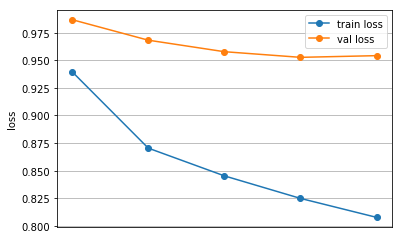
\includegraphics[width=\textwidth]{plot7}
  \caption{Training and Validation Loss for Model III}
\end{minipage}%
\hfill
\begin{minipage}{.4\textwidth}
  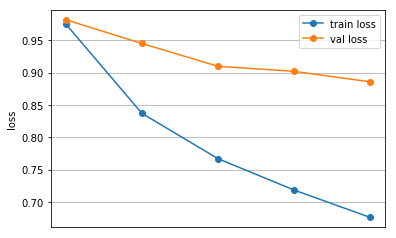
\includegraphics[width=\textwidth]{plot8}
  \caption{Training and Validation Loss for Model IV}
\end{minipage}
\end{figure}
\begin{figure}[]
\centering
\begin{minipage}{.4\textwidth}
  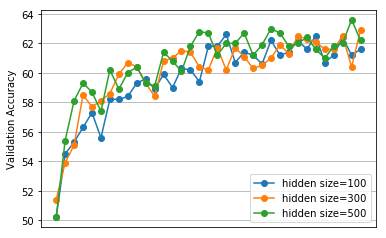
\includegraphics[width=\textwidth]{plot1}
  \caption{RNN Training Curve of 5 Epochs for Various Hidden Size}
\end{minipage}%
\hfill
\begin{minipage}{.4\textwidth}
  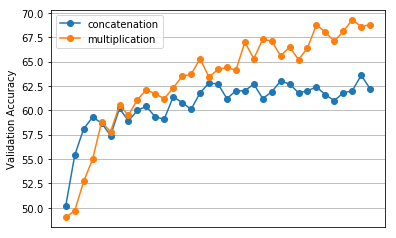
\includegraphics[width=\textwidth]{plot2}
  \caption{RNN Training Curve of 5 Epochs for Various Interaction Method}
\end{minipage}
\end{figure}

\paragraph{Vecter interaction Methods}
To further improve the performance of the model, the  paper experiments on the various way to interact the hidden representation of the two sentences. \textbf{Model IV} is built by multiplying the two encoded sentences element-wise. \textbf{Model IV} has parameter of size 3410003. The training loss and validation loss is ploted in Figure 4. The learning curve for the two models are ploted in Figure 6. \textbf{Model IV} shows significant improvement on the performance with accuracy of 70.4\%. Using different ways of interatcting vectors perserves different information from the hidden representation. By element-wise multiplying the two encoded vectors, the model incorperates the corresponding relationship between the two vectors. 

\paragraph{Correct and Incorrect Predictions}
Three correct predictions and three incorrect predictions are extracted from \textbf{Model IV}. The paper further evaluate the model through analyzing the reason of wrong prediction.\par
From the correct predictions especially the prediction 2, the bidirectional rnn model shows good performance in predicting the relationship between sentence even if information in the head of sentence 1 appear at the end of sentence 2. The model predicts well when the sentence structure changed.
While analyzing the incorrect predictions, the model show more false entailment prediction.  The unknown word tokens may affect the prediction in some way. Large number of similar word tokens will confuse the model to disregard the unknwon word token and incline to false entailment prediction.


Correct prediction 1:\par
\textit{sentence 1}: 'A', 'young', 'girl', 'with', 'blue', 'and', 'pink', 'ribbons', 'in', 'her', '<unk>', ',', 'without', 'a', 'top', 'and', 'a', 'woman', 'with', 'a', 'white', 't-shirt', 'and', 'a', 'zebra', 'skirt', 'wading', 'in', 'a', 'public', 'water', 'fountain', '.'\par
\textit{sentence 2}:['A', 'young', 'girl', '<unk>', 'a', 'sweater', \par
\textit{label}: contradiction

Correct prediction 2:\par
\textit{sentence 1}: 'A', 'woman', 'wearing', 'gray', 'pants', ',', 'a', 'white', 'blouse', 'and', 'a', 'black', 'vest', 'is', 'jumping', 'with', 'one', 'hand', 'in', 'the', 'air', 'as', 'she', 'goes', 'through', 'an', 'indoor', 'stadium', '.'\par
\textit{sentence 2}:'The', 'female', 'stadium', 'worker', 'jumps', 'for', 'joy', 'as', 'she', 'leaves', 'her', 'long', 'tiring', 'shift', '.'\par
\textit{label}: entailment\par
Correct prediction 3:\par
\textit{sentence 1}: 'A', 'young', 'woman', 'with', 'red', 'hear', 'and', 'wearing', 'a', 'bikini', 'top', 'is', 'standing', 'with', 'her', 'hands', 'together', 'above', 'her', 'head', ',', 'while', 'three', 'other', 'people', 'stand', 'directly', 'behind', 'her', 'with', 'their', 'arms', 'in', 'different', 'positions', ',', 'making', 'the', 'woman', 'in', 'front', 'look', 'as', 'if', 'she', 'has', 'many', 'arms', '.'\par
\textit{sentence 2}:'Some', 'people', 'are', 'holding', 'hands', 'and', 'walking', 'away', '.'\par
\textit{label}: contradiction\par

Incorrect prediction 1:\par
\textit{sentence 1}: 'A', 'man', 'in', 'a', 'brown', 'jacket', ',', 'white', 'shirt', ',', 'and', 'dark', '<unk>', 'is', 'holding', 'a', 'book', 'with', 'his', 'finger', 'on', 'the', 'page', 'while', 'sitting', 'on', 'a', 'wooden', 'floor', ',', 'and', 'leaning', 'against', 'a', 'yellow', 'wall', 'with', 'a', 'door', 'on', 'one', 'side', 'and', 'cloths', 'on', '<unk>', 'on', 'the', 'other', 'side', '.'\par
\textit{sentence 2}:'A', 'man', 'sits', 'on', 'a', 'wooden', 'floor', 'building', 'a', 'model', 'ship', '.'\par
\textit{label}: contradiction\par
\textit{predict}: entailment\par

Incorrect prediction 2:\par
\textit{sentence 1}: 'There', 'are', 'four', 'US', 'military', 'soldiers', 'in', 'this', 'photo', ',', 'only', 'two', 'have', 'their', 'faces', 'in', 'the', 'picture', ',', 'there', 'is', 'a', 'pack', 'of', 'cigarettes', 'by', 'one', 'of', 'their', 'boots', ',', 'they', 'appear', 'to', 'be', 'fixing', 'a', 'motorcycle', '.'\par
\textit{sentence 2}:'A', '<unk>', 'being', 'fixed', 'by', 'a', 'group', 'of', 'men', '.'\par
\textit{label}: neutral\par
\textit{predict}: entailment\par


Incorrect prediction 3:\par
\textit{sentence 1}: 'A', 'man', 'in', 'a', 'dark', 'suit', 'talks', 'with', 'a', 'middle-aged', 'man', 'and', 'woman', 'on', 'a', 'stage', 'in', 'front', 'of', 'a', 'large', 'logo', 'of', 'the', 'letter', '<unk>', 'D', '<unk>', 'with', 'the', 'numeral', 'five', 'within', 'it', '.'\par
\textit{sentence 2}:'A', 'couple', 'of', 'people', 'are', 'presenting', 'at', 'a', 'conference', '.'\par
\textit{label}: entailment\par
\textit{predict}: contradiction\par


\section{CNN Model}
In this section, the paper builds baseline model with a two-layer CNN as encoder for the pre-embeded input and feed them to two layers of fully connected neural networks. The hyperparameters, including the hidden layer size andthe kernal size.

\paragraph{Hidden Layers Size}
The paper experiment on three different size of hidden layers 200 \textbf{Model V}, 300 \textbf{Model VI}, 500 \textbf{Model VII}, 1000 \textbf{Model VIII}, . As explained in the last section, it is suspected that the higher hidden layer size would yield higher accuracy. Greater number of neurons in the network extracts more information from the input sentences for the model to process. Figure 3 shows as the hidden laye size increases, the accuracy improves though trivial. 
The Table 2 below shows the improvement on the accuracy versus the corresponding computational cost. For the current amount of training data, \textbf{Model VII} with hidden size 500 would be more practical. 

\begin{table}[]
\centering
\caption{My caption}
\label{my-label}
\begin{tabular}{lllll}
\hline
         & Hidden Size = 200 & Hidden Size = 300 & Hidden Size = 500 & Hidden Size = 1000 \\ \hline
Accuracy & 438.45            & 449.10            & 479.39            & 717.65             \\
Training Time     & 64.5              & 64.9              & 65.2              & 65.9               \\ \hline
\end{tabular}
\end{table}

\begin{figure}[h]
\centering
\begin{minipage}{.4\textwidth}
  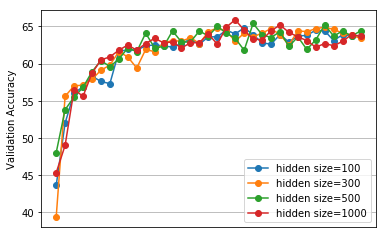
\includegraphics[width=\textwidth]{plot3}
  \caption{CNN Training Curve of 5 Epochs for Various Hidden Size}
\end{minipage}%
\hfill
\begin{minipage}{.4\textwidth}
  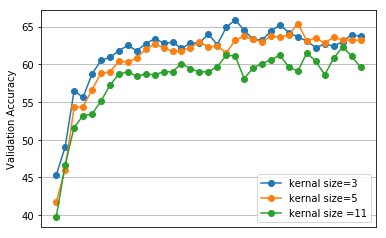
\includegraphics[width=\textwidth]{plot4}
  \caption{CNN Training Curve of 5 Epochs for Various Kernal Size}
\end{minipage}
\end{figure}

\paragraph{Kernal Size}
In CNN model application on nature language processing, the kernal size has the similar concept as the number of words in a bag for the N-gram model. The kernal size of 3, 5 and 11 [\textbf{Model VIII}, \textbf{Model IX},and  \textbf{Model X}] is trained to see the influence. The parameter size for all CNN model is shown in Table3. The learning curve is shwon in Figure 4. Figure 4 shows that the accuracy decreases as we increase the kernal size. As the kernal size increases, the probability of similar kernal decreases. Though larger kernal size should extract more precise information that incorperates the sentence environment, the sparsity issue causes the model performance to decrease. For much more training data, the large kernal size should yield great model.  Here we use large size of maxpooling kernal to find similar pattern within the sentence as complement in some degree.
\begin{table}[]
\centering
\caption{Number of Parameters for Model V, VI, VII, VIII, IX, X}
\label{my-label}
\begin{tabular}{lllllll}
\hline
                     & Model V & Model VI & Model VII & Model VIII & Model IX & Model X  \\ \hline
Number of Parameters & 161003  & 903003   & 2205003   & 7910003    & 10510003 & 18310003 \\ \hline
\end{tabular}
\end{table}
\paragraph{Correct and Incorrect Predictions}
Again, three correct and three incorrect perdictions are extracted from the best performin model  \textbf{Model VII}.\par
Going through the examples, it is clear that sentence 2 is much shorter in length compared to sentence 1. Two of the three correct predictions have obvious contradict words. For the incorrect predictions, three of them are labelled as entailment. This shows the model perform badly on the prediction of entailment sementic. Analyzing the incorrect sentence pairs, sentence 1 tends to be fairly long and complicated with subordinate clause and unknown word tokens. Sentence 2 changes use of words and reversting the structure of sentences causing the model to be confused in these cases.  By introducing larger vocabulary, and also expand the kernal size for may improve this issue.

Correct prediction 1:\par
\textit{sentence 1}: 'A', 'man', 'in', 'a', 'brown', 'jacket', ',', 'white', 'shirt', ',', 'and', 'dark', '<unk>', 'is', 'holding', 'a', 'book', 'with', 'his', 'finger', 'on', 'the', 'page', 'while', 'sitting', 'on', 'a', 'wooden', 'floor', ',', 'and', 'leaning', 'against', 'a', 'yellow', 'wall', 'with', 'a', 'door', 'on', 'one', 'side', 'and', 'cloths', 'on', '<unk>', 'on', 'the', 'other', 'side', '.'\par
\textit{sentence 2}:'A', 'man', 'sits', 'on', 'a', 'wooden', 'floor', 'building', 'a', 'model', 'ship', '.'\par
\textit{label}: contradiction\par
Correct prediction 2:\par
\textit{sentence 1}: 'Three', 'women', ',', 'two', 'wearing', 'red', 'shirts', 'and', 'one', 'wearing', 'a', 'purple', 'shirt', ',', 'and', 'a', 'man', ',', 'wearing', 'a', 'light', 'blue', 'shirt', ',', 'jump', 'on', 'a', 'basketball', 'court', 'with', 'balls', 'in', 'their', 'hands', '.'\par
\textit{sentence 2}:'Three', 'people', "'s", 'are', 'eating', 'in', 'hotel', '.'\par
\textit{label}: contradiction\par
Correct prediction 3:\par
\textit{sentence 1}: 'A', 'man', 'wearing', 'a', 'black', 'T-shirt', 'and', 'a', 'tan', 'jacket', 'wrapped', 'around', 'his', 'waist', 'pulls', 'a', 'wheeled', 'gray', 'and', 'black', 'bag', 'as', 'he', 'walks', 'next', 'to', 'a', 'building', 'that', 'has', 'large', 'glass', 'windows', '.'\par
\textit{sentence 2}:'A', 'person', 'walking', 'outside', '.'\par
\textit{label}: neutral\par

Incorrect prediction 1:\par
\textit{sentence 1}: 'A', '<unk>', 'woman', 'in', 'a', 'blue', 'top', 'and', 'black', '<unk>', 'looks', 'off', 'to', 'the', 'side', 'of', 'the', 'camera', 'with', 'a', 'drink', 'in', 'one', 'hand', 'and', 'a', 'amused', 'look', 'upon', 'her', 'face', ',', 'while', 'a', 'man', 'sits', 'next', 'to', 'her', ',', 'looking', '<unk>', ',', 'drink', 'in', 'one', 'hand', ',', 'straw', 'in', 'the', 'other', '.'\par
\textit{sentence 2}:['A', 'man', 'and', 'woman', 'are', 'having', 'drinks', 'in', 'a', 'bar', '.'\par
\textit{label}: entailment\par
\textit{predict}: contradiction\par

Incorrect prediction 2:\par
\textit{sentence 1}: 'Two', 'men', 'dressed', 'in', 'identical', 'white', 'jackets', 'with', 'green', 'numbers', 'and', 'logo', 'are', 'studying', 'something', 'on', 'a', 'cellphone', 'with', 'great', 'interest', ',', 'while', 'other', 'men', ',', 'identically', 'dressed', 'and', 'standing', 'in', 'a', 'group', 'with', 'these', 'two', ',', 'are', 'interested', 'in', 'something', 'to', 'their', 'right', '.'\par
\textit{sentence 2}:'Three', 'men', 'in', 'matching', 'jackets', 'are', 'standing', 'together', ',', 'one', 'looking', 'at', 'a', 'nearby', 'person', ',', 'the', 'other', 'two', 'looking', 'at', 'a', 'phone', '.'\par
\textit{label}: entailment\par
\textit{predict}: neutral\par


Incorrect prediction 3:\par
\textit{sentence 1}: 'A', 'young', 'boy', 'in', 'a', 'cowboy', 'hat', 'and', 'holding', 'some', 'food', 'sits', 'in', 'the', 'back', 'of', 'a', 'small', 'vehicle', 'while', 'an', 'adult', 'leans', 'over', 'in', 'the', 'background', 'next', 'to', 'a', 'large', 'blue', 'device', 'displaying', 'the', 'words', '99', '\%', 'Angel', '.'\par
\textit{sentence 2}:'A', 'young', 'boy', 'in', 'a', 'cowboy', 'hat', 'is', 'holding', 'a', 'hamburger', '.'\par
\textit{label}: entailment\par
\textit{predict}: neutral\par


\section{Comparison Between CNN and RNN}
Comparing between the incorrect predictions of the two best perform models, it reveals various advantage and disadvantage of the two models. RNN performs better when the sentences have structure reformed, while CNN model does not limit to the similarity of appeared words between two sentenses. The bidirectional feature of the RNN model and the max-pooling from CNN gives the two model their different characters.
The model would perform better if we interact CNN and RNN together to train.

\section{Multi-Natural Language Inference}
In this section, the paper deploys the best performed CNN and RNN model in the last two sections onto the Multi-natural Language Inference Task. Here we have five different genres (fiction, government, slate, telephone and travel) of data. The accuracies on the validation set will be plotted in a table below to analyze the influence of genre on the model performance.

\begin{table}[h]
\centering
\caption{Table for Multi-Natural Language Inference}
\label{my-label}
\begin{tabular}{lll}
\hline
 & RNN & CNN \\ \hline
SNLI Training Set & 68.8 & 65.2 \\
Genre 1: Fiction & 45.13 & 42.21 \\
Genre 2: Government & 43.21 & 39.57 \\
Genre 3: Slate & 41.41 & 39.92 \\
Genre 4: Telephone & 43.98 & 41.49 \\
Genre 5: Travel & 43.58 & 41.24 \\ \hline
\end{tabular}
\end{table}

From Table 4, it is clear that applying the trained model to unfamiliar genres yield poor accuracy. All accuracies are below 50\% which is even lower than random model. The phenomenon proves that the nlp model is highly dependent on the genre on the training data. Comparing column-wise through the table, some genre have correlation between each other. For example, both model performs slightly better for 'fiction' as it is closer to our novel training set. Models perform badly on 'government' and 'slate', since they have very different style, being more precise and rigorous.



\section{Appendix}
All the python code are uploaded to github as jupyter notebook file at the following link:
\url{https://github.com/nicoleqiwt/NLP1011-SNLI.git}

\end{document}
